\fancychapter{Introduction}
\cleardoublepage
\label{chapter:1}
% What is language and speech
The faculty of expressing or describing thoughts, feelings and needs by using language is a fundamental ability in our daily lives. The process of language production involves the organisation of words joined in a meaningful manner. Effective communication through language begins with the conceptualization of the message to be transmitted (\textit{conceptualisation}), followed by the selection of appropriate lexical items and subsequent grammatical encoding (\textit{formulation}). Subsequently, the linguistic representation is transformed into sound through the transmission of this representation from the brain to the muscles of the complex speech system including lips, larynx, glottis, lungs, jaw and tongue (\textit{articulation}) \cite{levelt1993speaking}.

% Children speech and language acquisition
The capability to speak and comprehend language is not inherently present but rather develops gradually over time with experience. Typically, children reach specific language milestones at particular ages. For example, around 12 to 18 months, a child usually utters their first words and starts imitating sounds. By the age of 4 to 5, children tend to formulate sentences and grasp more intricate concepts. Regarding speech sounds, younger children, approximately 1 year old, can produce basic speech sounds like \textit{/p/}, \textit{/b/}, \textit{/m/} while older children, around 5 years old, can articulate more complex sounds such as \textit{/r/} and \textit{/th/}. This developmental stage is referred as language acquisition, and it plays a crucial role in a child's overall development. As individuals, our daily dependence on social and communication skills endures throughout our entire lives. Consequently, it is imperative for children to develop the capacity to interact effectively with others to achieve seamless integration into society across all aspects of their lives.

% But pathology exists, need for therapy/assessment
Regrettably, a subset of children experience speech disorders stemming from congenital conditions such as cleft palate, cerebral palsy, and prelingual deafness. Alternatively, certain individuals may acquire speech-related issues during childhood, encompassing cognitive developmental delays, breathing-feeding-swallowing disorders and traumatic brain injuries. Notably, in 2012, empirical data \cite{black2015communication} highlighted that 7.7\% of children aged 3 to 17 in the United States exhibited communication disorders, with 5.0\% of this cohort specifically presenting speech-related problems.

Furthermore, additional observation \cite{langbecker2020long} suggests that individuals afflicted with childhood speech disorders may confront an increased prevalence of mental health challenges, diminished social well-being, and reduced academic accomplishments in comparison to their peers. This underscores the intricate nature of childhood speech disorders, the repercussions of which extend into adolescence and adulthood. Hence,  early identification and intervention play a pivotal role in mitigating the enduring effects on these children's social interactions, communication skills, educational progress, and overall well-being.

% Speech therapy
Pediatric Speech and Language Pathologists (SLPs) play a crucial role in providing therapy to help children overcome the effects of speech disorders and offer early diagnosis. The therapy typically includes exercises and assessments, which can be based on perceptual speech evaluations or standardised tests. To effectively engage children, these activities are often presented as games, taking into consideration the inherently limited attention span of children. Notably, SLPs frequently maintain long-term follow-ups with their patients, allowing them to monitor the evolution of speech quality over time and tailor exercises to the specific needs of each child. The adoption of this individualised therapeutic approach is essential for helping children achieve improved speech and communication skills.

% problems with speech therapy (hospital, stress, ...)
Nevertheless, notwithstanding the valuable benefits offered by speech therapy, its pursuit can present a substantial financial and time investment for parents. Additionally, parents frequently find themselves lacking of training and expertise to provide their children with the more intricate exercises needed for further continued improvement in a home environment. Moreover, the hospital environment can induce stress in children. Lastly, it is important to acknowledge that, despite professional training, inter-expert variability in perceptual assessments may exist, giving rise to disparate diagnostic conclusions.

\begin{figure}
    \centering
    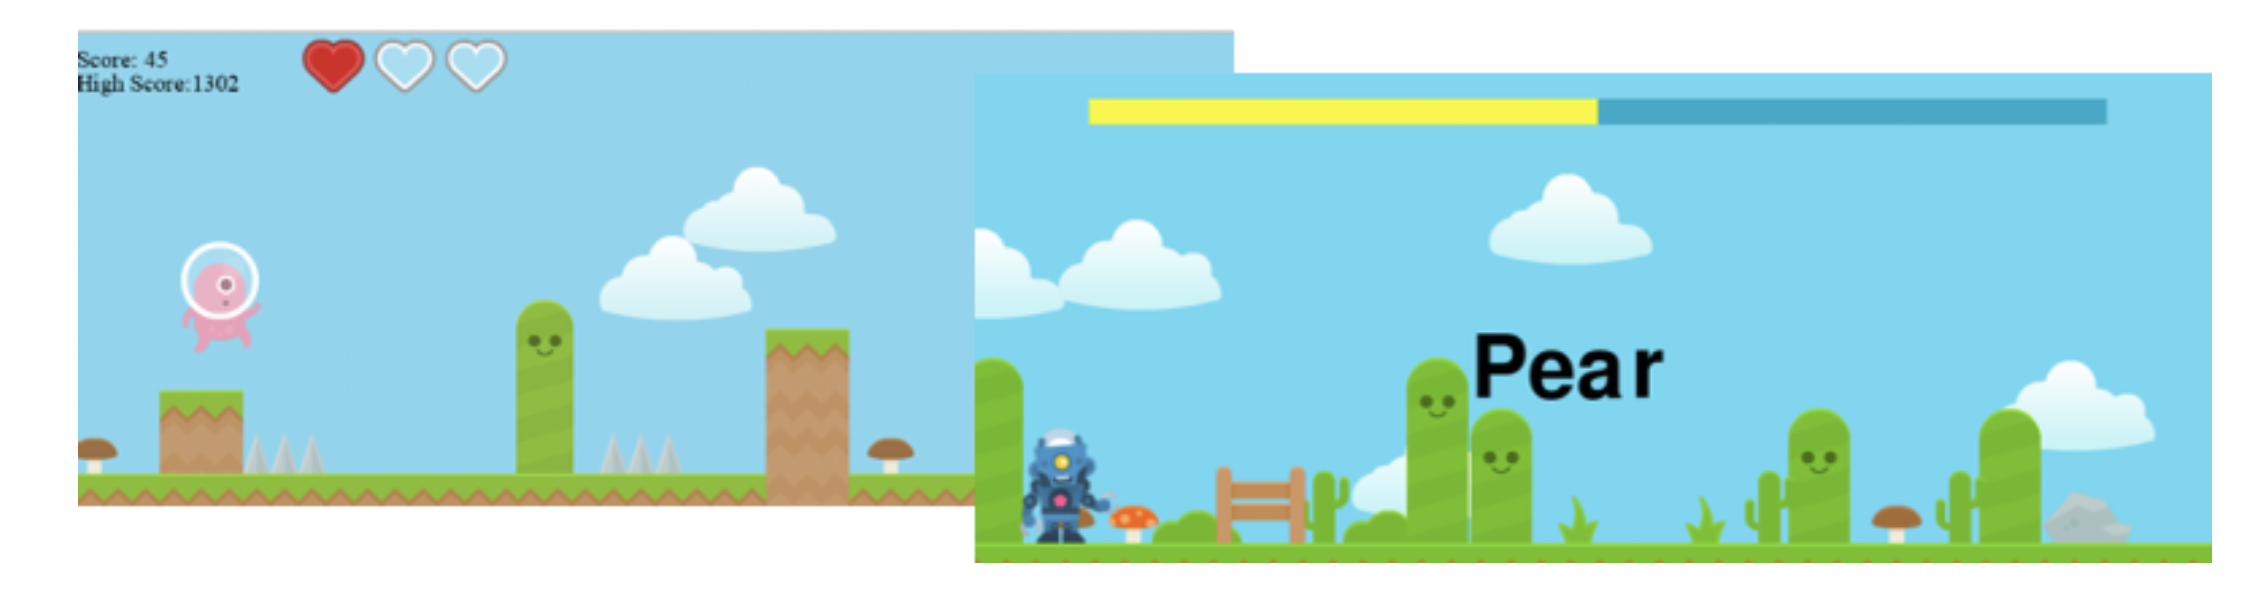
\includegraphics[width=1\textwidth]{imgs/exampleSLT.png}
    \caption{Illustrated herein are some examples of children's Speech and Language Technology applications that were developed during the course of this thesis. On the left is a running platformer game, where the user's voice controls the character. Pitch dictates running and jumping actions, while energy modulates the velocity of these actions. On the right, a reading task game is depicted, wherein a robot instructs the user to read designated words.}
    \label{fig:exSLT}

\end{figure}

% SLT could be the beginning of the answer and is already used in real life
In this context, Speech and Language Technologies (SLT) have arisen as highly pertinent within the domain of speech therapy. These technologies provide objective and precise automated assessments. Another benefit lies in their potential integration into gamification frameworks, thereby augmenting children's involvement during therapy. Several SLT examples developed within the scope of this thesis are illustrated in Figure \ref{fig:exSLT}. Moreover, the ability to record speech utter by the patient during a session using SLT enables thorough analysis and long-term monitoring post-session by the therapist. Due to the aforementioned reasons, the development of such tools has gained considerable attention, empowering patients to engage in exercises beyond therapy sessions, notably in a home setting.

\section{Problem statement}
% Technologies are more and more present
Recent years have seen an increased integration of SLT into various aspects of our daily lives, impacting a wide range of environments, including homes, transportation, education, and even the military. Noteworthy examples encompass voice assistants, hands-free computing, healthcare systems, automatic helplines, and speech-to-speech translation services. The progress in these applications has been made possible through the use of deep learning techniques, the increasing computational capacities of our devices, and the ever-growing volume of data available to train and improve these systems.

% Automatic tools for speech therapy
As previously mentioned, SLTs are gradually making their way into the field of atypical speech, particularly for children. While these automatic tools are currently in their early stages and have limitations, there is indeed a rising interest in implementing atypical speech and language therapy cutting-edge systems with a focus on assisting SLPs. In this context, systems that can automatically assess pronunciation quality and detect pathological speech conditions could be highly valuable in supporting pediatric SLPs. In addition, the ability of children with speech disorders to directly interact with machines using speech could prove to be a valuable tool in their daily lives.

All of these objectives require the implementation of an effective children's automatic speech recognition (ASR) system. However, while speech recognition technologies have made substantial advancements, leading to increased accuracy, the performance of ASR systems for children remains underperforming when compared to those for adults. This discrepancy results in unreliable systems for children's speech. The diminished performance can be ascribed to a combination of factors, including intra- and inter-speaker variability, limited linguistic and phonetic knowledge, and the scarcity of available data.

%This thesis aligns with this aspiration, aiming to provide the necessary tools for the development of an effective automatic speech recognition (ASR) system. Moreover, it's worth noting that most automatic pronunciation quality assessment systems primarily rely on automatic speech recognition

% In this work we propose....
Therefore, the aim of this thesis is to explore ways to enhance children's ASR in order to develop a robust foundational system that can be deployed effectively for children with speech pathologies.
% Area of interest of this work (for the ASR part)
%In order to achieve this objective, we have identified two main areas of interest which are presented in more detail hereafter:
%\begin{itemize}
%    \item Many improvements in ASR have been achieved by changing the system architecture and training procedures. However, these adjustments have not been designed for children. It is therefore important to study the influence of the different components and training procedures on the ASR performances of children. 
%    \item Children's speech data is much more difficult and unique to work with. As a result, research into data-driven strategies such as data augmentation and normalisation might aid in closing the ASR gap between children and adults.
%\end{itemize}
For that purpose, we list a few precise research questions that this thesis aims to address:
\begin{enumerate}
\item Which knowledge transfer approach is best for efficiently modelling and improving automatic recognition of children's speech? Can these approaches be used to efficiently exploit low-resource children's speech data from multiple languages?
\item  Why do end-to-end automatic speech recognition models achieve state-of-the-art results for children's ASR? Particularly, what are the components that are most important to fine-tune?
\item Is it possible to develop an age-based, parameter-efficient automatic speech recognition model?
\item Is it possible to use children's synthetic speech to extend the amount of children's data? How can we control the quality and speakers’ variability?
\item Given that self-supervised representation-based ASR for adults matches or surpasses current state-of-the-art, can these representations be appropriate for children’s speech also?
\end{enumerate}

\section{Contributions}
As mentioned in the previous section, SLT can assist paediatric speech therapists by automatically assessing pronunciation quality and identifying pathological conditions. Although the primary aim of this thesis was to improve ASR for reliable assessment of pronunciation quality. We also contributed to the identification of pathological conditions from speech, which will be discussed in this section. 

The potential of speech as a non-invasive biomarker for evaluating a speaker's health for both physical and psychological disorders has repeatedly been proven by the results of several works  \cite{hauptman2019identifying,botelho2019speech}. Traditional speech-based disease classification systems have focused on carefully researched, knowledge-based features. However, these features do not always capture the full disease's symptomatology and may even ignore some of its more subtle signs. This has led research to move towards generic representations that intrinsically model the symptoms. However, there are not enough pathological speech data available to train a large model directly. In our work \cite{botelho2020pathological}, we proposed to assess speaker embedding, such as \textit{i-vectors} \cite{ivector} and \textit{x-vectors} \cite{snyder2018x}, applicability as a generic feature extraction method to the detection of Parkinson’s disease (PD) and Obstructive Sleep Apnea (OSA). All disease classifications were performed with a support-vector-machine (SVM) classifier. Our experiments with European Portuguese datasets support the hypothesis that discriminative speaker embeddings contain information relevant to disease detection. In particular, we found evidence that these embeddings contain information that hand-crafted features fail to represent, thus proving the validity of our approach. It was also observed that x-vectors are more suitable than i-vectors for tasks whose domain does not match the training data, such as verbal task mismatch and cross-lingual. This indicates that x-vectors embeddings are a strong contender in the replacement of knowledge-based feature sets for PD and OSA detection.

Later, in \cite{pompili2020inesc}, we proposed to extend the aforementioned work by classifying Alzheimer's disease with the conjunction of both acoustic and textual feature embeddings. In this end, speech signals are encoded into \textit{x-vector} using pre-trained models. For textual input, contextual embedding vectors are first extracted using an English Bert model \cite{Bert} and then used to feed a bidirectional recurrent neural network with attention. This multi-model system, based on the combination of linguistic and acoustic information, attained a classification accuracy of 81.25\%. Results have shown the importance of linguistic features in the classification of Alzheimer’s disease, which outperforms the acoustic ones in terms of accuracy.

Finally, we further extend the idea of using pre-trained representation to automatically detect COVID-19 from cough recordings. We leverage transfer learning to develop a set of COVID-19 classification subsystems based on deep cough representation extractors called experts. Individual decisions of three experts are fed to a calibrated decision-level fusion system. This ensemble of expert subsystems based on cough representations is expected to produce well-calibrated log-likelihood scores over a wide range of operating points. The output can be more easily interpreted by a human expert and incorporated into the decision-making process. Our results show competitive performance compared to hand-crafted features, although they are still far from those required to become a reliable tool to assist COVID-19 screening.


\section{Structure for the thesis}

%In Chapter \ref{chap:Chapter2}, we survey related work relevant to this proposal. First, we explain how children's speech differs from adults' speech in terms of frequency, language, and available data. We then present a brief summary of automatic speech recognition systems and the most recent approaches to solving children's automatic speech recognition challenges. In Chapter \ref{chapter:Hybrid}, we present our work done on the hybrid speech recognition framework, while in Chapter \ref{chap:e2e} we present the work based on end-to-end models. Finally, in Chapter \ref{chap:final} we discuss the current and future work and the associated timeline.
